\chapter{EM 算法}\label{chapter:11}

本章将讨论用于密度估计的 EM(期望最大化)算法。

\section{面向高斯混合模型的 EM 算法}

假设像往常一样给定一个训练集 $\{x^{(1)}, \dots, x^{(n)}\}$。由于处于无监督学习设置中,这些点没有标签。

我们希望通过指定联合分布 $p(x^{(i)}, z^{(i)}) = p(x^{(i)}|z^{(i)})p(z^{(i)})$ 来建模数据。这里,$z^{(i)} \sim \text{Multinomial}(\phi)$(其中 $\phi_j \geq 0, \sum_{j=1}^k \phi_j = 1$,参数 $\phi_j$ 代表了 $p(z^{(i)} = j)$ 的值),并且 $x^{(i)}|z^{(i)} = j \sim \mathcal{N}(\mu_j, \Sigma_j)$。令 $k$ 表示 $z^{(i)}$ 可以取的值的数量。因此,我们的模型假设每个 $x^{(i)}$ 是通过从 $\{1, \dots, k\}$ 中随机选择 $z^{(i)}$ 生成的,然后 $x^{(i)}$ 是根据 $z^{(i)}$ 从 $k$ 个高斯分布中的一个中抽取的。这被称为\textbf{高斯混合 (mixture of Gaussians)} 模型。另请注意 $z^{(i)}$ 是\textbf{隐 (latent)} 变量,这意味着它们是隐藏/未观察到的。这使得我们的估计问题变得困难。

因此,模型的参数是 $\phi, \mu$ 和 $\Sigma$。为了估计它们,可以写出数据的似然函数:
\begin{align*}
    \ell(\phi, \mu, \Sigma) &= \sum_{i=1}^n \log p(x^{(i)}; \phi, \mu, \Sigma) \\
    &= \sum_{i=1}^n \log \sum_{z^{(i)}=1}^k p(x^{(i)}|z^{(i)}; \mu, \Sigma)p(z^{(i)}; \phi).
\end{align*}
然而,如果我们将此公式里的参数的导数设为 0 并尝试求解,会发现无法找到参数的闭式最大似然估计。(可以自行尝试。)

随机变量 $z^{(i)}$ 表示每个 $x^{(i)}$ 来自 $k$ 个高斯分布中的哪一个。注意,如果已知 $z^{(i)}$ 的值,最大似然问题是很容易的。具体来说,可以写出似然函数为
\[
    \ell(\phi, \mu, \Sigma) = \sum_{i=1}^n \log p(x^{(i)}|z^{(i)}; \mu, \Sigma) + \log p(z^{(i)}; \phi).
\]
对上式关于 $\phi, \mu$ 和 $\Sigma$ 求最大值,得到参数:
\begin{align*}
    \phi_j &= \frac{1}{n} \sum_{i=1}^n 1\{z^{(i)} = j\},\\
    \mu_j &= \frac{\sum_{i=1}^n 1\{z^{(i)} = j\}x^{(i)}}{\sum_{i=1}^n 1\{z^{(i)} = j\}},\\
    \Sigma_j &= \frac{\sum_{i=1}^n 1\{z^{(i)} = j\}(x^{(i)} - \mu_j)(x^{(i)} - \mu_j)^T}{\sum_{i=1}^n 1\{z^{(i)} = j\}}.
\end{align*}

确实,可以看到,如果已知 $z^{(i)}$ 的值,那么最大似然估计几乎与估计高斯判别分析模型的参数完全相同,不同之处在于这里 $z^{(i)}$ 扮演着类别标签的角色。\footnote{这里的公式与在习题集 1 中高斯判别分析的公式有一些细微差别,首先是因为我们将 $z^{(i)}$ 推广为多项分布而不是伯努利分布,其次是因为这里我们对每个高斯分布使用不同的 $\Sigma_j$。}

但是在密度估计问题中,$z^{(i)}$ 的值是未知的。该怎么办?

EM 算法是一种迭代算法,它有两个主要步骤。在步骤 E 中,它尝试“猜测”$z^{(i)}$ 的值。在步骤 M 中,它根据我们的猜测更新模型的参数。由于在步骤 M 中假装第一部分的猜测是正确的,最大化就变得容易了。以下是算法:

重复直到收敛:\{
    \begin{itemize}
        \item[] \quad(步骤 E) 对于每个 $i, j$,设置
            \[
                w_j^{(i)} := p(z^{(i)} = j | x^{(i)}; \phi, \mu, \Sigma)
            \]
        \item[] \quad(步骤 M) 更新参数:
            \begin{align*}
                \phi_j &:= \frac{1}{n} \sum_{i=1}^n w_j^{(i)},\\
                \mu_j &:= \frac{\sum_{i=1}^n w_j^{(i)} x^{(i)}}{\sum_{i=1}^n w_j^{(i)}},\\
                \Sigma_j &:= \frac{\sum_{i=1}^n w_j^{(i)} (x^{(i)} - \mu_j)(x^{(i)} - \mu_j)^T}{\sum_{i=1}^n w_j^{(i)}}
            \end{align*}
    \end{itemize}

\}

在步骤 E 中,根据给定的 $x^{(i)}$ 和当前参数设置,计算参数 $z^{(i)}$ 的后验概率。也就是说,使用贝叶斯法则,得到:
\[
    p(z^{(i)} = j | x^{(i)}; \phi, \mu, \Sigma) = \frac{p(x^{(i)}|z^{(i)} = j; \mu, \Sigma)p(z^{(i)} = j; \phi)}{\sum_{l=1}^k p(x^{(i)}|z^{(i)} = l; \mu, \Sigma)p(z^{(i)} = l; \phi)}
\]
其中,$p(x^{(i)}|z^{(i)} = j; \mu, \Sigma)$ 是在 $x^{(i)}$ 处计算均值为 $\mu_j$、协方差为 $\Sigma_j$ 的高斯分布的密度函数;$p(z^{(i)} = j; \phi)$ 由 $\phi_j$ 给出,依此类推。在步骤 E 中计算的 $w_j^{(i)}$ 值代表了对 $z^{(i)}$ 值的“软”猜测。\footnote{“软”指的是猜测是概率且取值在 $[0, 1]$ 中;作为对比,“硬”表示单一的最佳猜测(例如取值在 $\{0, 1\}$ 或 $\{1, \dots, k\}$ 中)。}

此外,应该将步骤 M 中的更新公式与已知 $z^{(i)}$ 值时的公式进行对比。它们是相同的,只不过前面使用指示函数 $1\{z^{(i)} = j\}$ 表示每个数据点来自哪个高斯分布,而这里使用 $w_j^{(i)}$。

EM 算法也让人联想到 K-means 聚类算法,不同之处在于 K-means 使用“硬”聚类分配 $c(i)$,而这里使用“软”分配 $w_j^{(i)}$。与 K-means 类似,EM 算法也容易陷入局部最优,因此使用几个不同的初始参数进行重新初始化可能是个好主意。

显然,EM 算法对重复猜测未知 $z^{(i)}$ 值具有非常自然的解释;但是它是如何得出的?我们能对其做出任何保证吗,例如关于其收敛性?后面我们将更一般地描述 EM 算法,使得该算法更容易应用于其他包含隐变量的估计问题,并使其收敛性得到保证。

\section{Jensen 不等式}

我们从一个非常有用的结果开始讨论,即 \textbf{Jensen 不等式 (Jenson's inequality)}。

设 $f$ 是一个定义域为实数集的函数。回想一下,当 $f''(x) \geq 0$ 时 $f$ 是一个凸函数(对于所有 $x \in \mathbb{R}$)。对于取向量值输入的函数,这推广为其 Hessian 矩阵 $H$ 是半正定 ($H \geq 0$) 的条件。如果对于所有 $x$,都有 $f''(x) > 0$,则称 $f$ 为\textbf{严格 (strictly)} 凸函数(在向量值情况下,相应的表述是 $H$ 必须是正定的,记作 $H > 0$)。Jensen 不等式可以表述如下:

\begin{theorem*}
    设 $f$ 是一个凸函数,且 $X$ 是一个随机变量。则:
    \[
        \mathrm{E}[f(X)] \geq f(\mathrm{E}X).
    \]
    此外,如果 $f$ 是严格凸函数,则 $\mathrm{E}[f(X)] = f(\mathrm{E}X)$ 当且仅当 $X = \mathrm{E}[X]$ 以概率 1 成立(即 $X$ 是一个常数)。
\end{theorem*}

回想一下,在书写期望时,有时会省略括号,因此在上述定理中,$f(\mathrm{E}X) = f(\mathrm{E}[X])$。

对于该定理的解释,请参考下图。

\begin{figure}[H]
    \centering
    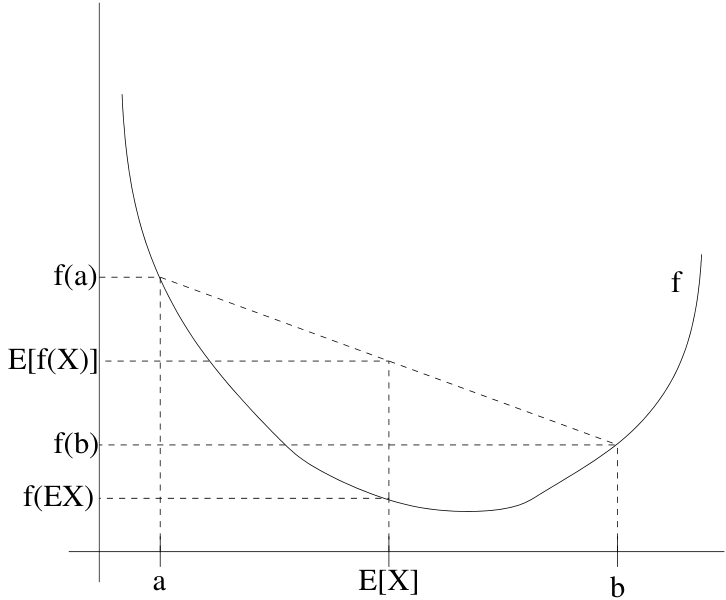
\includegraphics[width=0.6\textwidth]{figs/Jenson_inequality.png}
\end{figure}

此处,$f$ 是由实线表示的凸函数。$X$ 是一个随机变量,其取值 $a$ 的概率为 0.5,取值 $b$ 的概率为 0.5(在 $x$ 轴上标示)。因此,$X$ 的期望值是 $a$ 和 $b$ 的中点。

还可以在 $y$ 轴上看到 $f(a)$、$f(b)$ 和 $f(\mathrm{E}[X])$ 的值。此外,值 $\mathrm{E}[f(X)]$ 现在是 $y$ 轴上 $f(a)$ 和 $f(b)$ 之间的中点。从示例中,我们看到因为 $f$ 是凸函数,所以必然有 $\mathrm{E}[f(X)] \geq f(\mathrm{E}X)$。

顺便说一句,很多人在记忆不等式的方向时会遇到困难,记住这个图是一个快速得出答案的好方法。

\begin{remark*}
    回想一下,$f$ 是(严格)凹函数当且仅当 $-f$ 是(严格)凸函数(即 $f''(x) \leq 0$ 或 $H \leq 0$)。Jensen 不等式对于凹函数 $f$ 也成立,但所有不等号的方向都反转了(如 $\mathrm{E}[f(X)] \leq f(\mathrm{E}X)$)。
\end{remark*}

\section{广义 EM 算法}

假设有一个估计问题,其包含一个有 $n$ 个独立样本的训练集 $\{x^{(1)}, \dots, x^{(n)}\}$。我们有一个隐变量模型 $p(x, z; \theta)$,其中 $z$ 是隐变量(为简单起见,假设其取有限个值)。$x$ 的密度可以通过对隐变量 $z$ 进行边缘化得到:
\begin{equation}
    p(x; \theta) = \sum_z p(x, z; \theta)
    \label{eq:11.1}
\end{equation}

我们希望通过最大化数据的对数似然来拟合参数 $\theta$,对数似然定义为:
\begin{equation}
    \ell(\theta) = \sum_{i=1}^n \log p(x^{(i)}; \theta)
    \label{eq:11.2}
\end{equation}
可以将目标函数写成联合密度 $p(x, z; \theta)$ 的形式:
\begin{align}
    \ell(\theta) 
    &= \sum_{i=1}^n \log p(x^{(i)}; \theta) \label{eq:11.3} \\
    &= \sum_{i=1}^n \log \sum_{z^{(i)}} p(x^{(i)}, z^{(i)}; \theta). \label{eq:11.4}
\end{align}
但是,显式地找到参数 $\theta$ 的最大似然估计可能很困难,因为它会导致困难的非凸优化问题。\footnote{这个优化问题难以优化主要是一种经验性的观察。}这里,$z^{(i)}$ 是隐随机变量;通常情况下,如果 $z^{(i)}$ 被观测到,那么最大似然估计就会变得容易。

在这种设置下,EM 算法提供了一种有效的最大似然估计方法。显式地最大化 $\ell(\theta)$ 可能很困难,因此我们的策略是反复构造一个 $\ell(\theta)$ 的下界(步骤 E),然后优化该下界(步骤 M)。\footnote{根据经验,步骤 E 和步骤 M 通常比直接优化函数 $\ell(\cdot)$ 更高效。然而,这并不一定意味着交替执行这两个步骤总能收敛到 $\ell(\cdot)$ 的全局最优解。即使对于高斯混合模型,EM 算法也可能收敛到全局最优解或陷入局部最优,这取决于训练数据的性质。根据经验,对于实际数据,EM 通常可以收敛到具有相对高似然的解(即使不是最优解),其背后的理论很大程度上尚未被完全理解。}

事实证明,这里的求和 $\sum_{i=1}^n$ 并非本质的。为了更简单地阐述 EM 算法,首先考虑对\textbf{单个样本 (a single example)} $x$ 的似然 $\log p(x)$ 进行优化。在推导出优化 $\log p(x)$ 的算法后,我们将通过将相关方程相加来将其转换为适用于 $n$ 个样本的算法。因此,现在我们要优化 $\log p(x; \theta)$,它可以重写为
\begin{equation}
    \log p(x; \theta) = \log \sum_z p(x, z; \theta)
    \label{eq:11.5}
\end{equation}
令 $Q$ 是 $z$ 可能取值上的一个分布。也就是说,$\sum_z Q(z) = 1$,且 $Q(z) \geq 0$。

考虑以下推导:\footnote{如果 $z$ 是连续变量,则 $Q$ 是一个概率密度函数,对 $z$ 的求和也变为对 $z$ 的积分。}
\begin{align}
    \log p(x; \theta) &= \log \sum_z p(x, z; \theta) \nonumber \\
    &= \log \sum_z Q(z) \frac{p(x, z; \theta)}{Q(z)}
    \label{eq:11.6} \\
    &\geq \sum_z Q(z) \log \frac{p(x, z; \theta)}{Q(z)}
    \label{eq:11.7}
\end{align}

上述推导的最后一步使用了 Jensen 不等式。具体来说,$f(x) = \log x$ 是一个凹函数,因为在其定义域 $x\in \mathbb{R}^+$ 上 $f''(x) = -1/x^2 < 0$。此外,求和项
\[
    \sum_z Q(z) \left[ \frac{p(x, z; \theta)}{Q(z)} \right]
\]
是 $[p(x, z; \theta)/Q(z)]$ 关于从分布 $Q$ 抽取的 $z$ 的期望。\footnote{注意到,当 $p(x, z; \theta) \neq 0$ 时,表达式 $\frac{p(x, z; \theta)}{Q(z)}$ 只有在 $Q(z) \neq 0$ 时才有意义。在此,隐含地假设只考虑满足这一性质的 $Q$。} 根据 Jensen 不等式,有
\[
    f\left( \mathbb{E}_{z \sim Q}\left[ \frac{p(x, z; \theta)}{Q(z)} \right] \right) \geq \mathbb{E}_{z \sim Q}\left[ f\left( \frac{p(x, z; \theta)}{Q(z)} \right) \right],
\]
其中下标标“$z \sim Q$”表示期望是关于从 $Q$ 中抽取的 $z$ 计算的。这使得公式 \eqref{eq:11.6} 可以推导到公式 \eqref{eq:11.7}。

现在,对于任何分布 $Q$,公式 \eqref{eq:11.7} 给出了 $\log p(x; \theta)$ 的一个下界。对于 $Q$ 有许多可能的选择,应该选择哪一个呢?如果对参数 $\theta$ 有当前的猜测值,那么自然会尝试使该下界在 $\theta$ 的该值处尽可能紧。也就是说,希望在 $\theta$ 的特定值处使上述不等式取等号。为了上述推导中涉及 Jensen 不等式的步骤取等号,需要期望作用在一个“常数值”随机变量上。也就是说,要求对于某个不依赖于 $z$ 的常数 $c$,有
\[
    \frac{p(x, z; \theta)}{Q(z)} = c
\]
这很容易通过选择
\[
    Q(z) \propto p(x, z; \theta)
\]
来实现。
实际上,由于 $\sum_z Q(z) = 1$(因为它是一个分布),这进一步揭示了
\begin{align}
    Q(z) &= \frac{p(x, z; \theta)}{\sum_z p(x, z; \theta)}
    \nonumber\\
    &= \frac{p(x, z; \theta)}{p(x; \theta)} 
    \nonumber\\
    &= p(z|x; \theta)
    \label{eq:11.8}
\end{align}
因此,将 $Q$ 设置为给定 $x$ 和参数 $\theta$ 下 $z$ 的后验分布。

事实上,当 $Q(z) = p(z|x; \theta)$ 时,可以直接验证公式 \eqref{eq:11.7} 是一个等式,因为
\begin{align*}
    \sum_z Q(z) \log \frac{p(x, z; \theta)}{Q(z)} &= \sum_z p(z|x; \theta) \log \frac{p(x, z; \theta)}{p(z|x; \theta)} \\
    &= \sum_z p(z|x; \theta) \log \frac{p(x, z; \theta) p(x; \theta)}{p(z|x; \theta) p(x; \theta)} \\
    &= \sum_z p(z|x; \theta) \log p(x; \theta) \\
    &= \log p(x; \theta) \sum_z p(z|x; \theta) \\
    &= \log p(x; \theta) \quad (\text{因为 } \sum_z p(z|x; \theta) = 1)
\end{align*}

为方便起见,将公式 \eqref{eq:11.7} 中的表达式称为 \textbf{证据下界 (evidence lower bound, ELBO)},并用下式表示:
\begin{equation}
    \text{ELBO}(x; Q, \theta) = \sum_z Q(z) \log \frac{p(x, z; \theta)}{Q(z)}
    \label{eq:11.9}
\end{equation}
根据这个等式,可以将公式 \eqref{eq:11.7} 重写为
\begin{equation}
    \forall Q, \theta, x, \quad \log p(x; \theta) \geq \text{ELBO}(x; Q, \theta)
    \label{eq:11.10}
\end{equation}
直观上,EM 算法通过以下方式交替更新 $Q$ 和 $\theta$:a) 根据公式 \eqref{eq:11.8} 设置 $Q(z) = p(z|x; \theta)$,从而使 $\text{ELBO}(x; Q, \theta) = \log p(x; \theta)$ 对于 $x$ 和当前的 $\theta$ 成立;b) 在固定 $Q$ 的选择下,最大化 $\text{ELBO}(x; Q, \theta)$ 关于 $\theta$ 的值。

回想一下,上述所有讨论都是在优化单个样本 $x$ 的对数似然 $\log p(x; \theta)$ 的假设下进行的。事实证明,对于多个训练样本,基本思想是相同的,只需要在相关位置对样本进行求和即可。接下来将构建针对多个训练样本的证据下界,并使 EM 算法形式化。

我们有一个训练集 $\{x^{(1)}, \dots, x^{(n)}\}$。注意,$Q$ 的最优选择是 $p(z|x; \theta)$,它取决于特定的样本 $x$。因此,在这里将对于每个样本 $x^{(i)}$ 引入 $n$ 个分布 $Q_1, \dots, Q_n$,从而构建证据下界
\[
    \log p(x^{(i)}; \theta) \geq \text{ELBO}(x^{(i)}; Q_i, \theta) = \sum_{z^{(i)}} Q_i(z^{(i)}) \log \frac{p(x^{(i)}, z^{(i)}; \theta)}{Q_i(z^{(i)})}
\]
对所有样本求和,可以得到对数似然的下界
\begin{align}
    \ell(\theta) 
    &\geq \sum_i \text{ELBO}(x^{(i)}; Q_i, \theta) \label{eq:11.11}\\
    &= \sum_i \sum_{z^{(i)}} Q_i(z^{(i)}) \log \frac{p(x^{(i)}, z^{(i)}; \theta)}{Q_i(z^{(i)})} \nonumber
\end{align}

对于\textit{任意 (any)} 一组分布 $Q_1, \dots, Q_n$,公式 \eqref{eq:11.11} 给出了 $\ell(\theta)$ 的一个下界,并且与公式 \eqref{eq:11.8} 的论证类似,达到等号的 $Q_i$ 满足
\[
    Q_i(z^{(i)}) = p(z^{(i)}|x^{(i)}; \theta)
\]
因此,将 $Q_i$ 设置为给定 $x^{(i)}$ 和当前参数 $\theta$ 设置下 $z^{(i)}$ 的后验分布。

现在,对于 $Q_i$ 的这种选择,公式 \eqref{eq:11.11} 给出了试图最大化的对数似然 $\ell$ 的下界。这是步骤 E。算法的步骤 M 将最大化公式 \eqref{eq:11.11} 中关于参数的表达式,从而获得 $\theta$ 的新设置。重复执行这两个步骤就得到了 EM 算法,其过程如下:

重复直到收敛 \{
    \begin{itemize}
        \item[] \quad(步骤 E) 对于每个 $i$,设置
        \[
            Q_i(z^{(i)}) := p(z^{(i)}|x^{(i)}; \theta).
        \]
        \item[] \quad(步骤 M) 设置
        \begin{align}
            \theta &:= \arg\max_\theta \sum_{i=1}^n \text{ELBO}(x^{(i)}; Q_i, \theta) \nonumber\\
            &= \arg\max_\theta \sum_i \sum_{z^{(i)}} Q_i(z^{(i)}) \log(p(x^{(i)}, z^{(i)}; \theta) / Q_i(z^{(i)})).\label{eq:11.12}
        \end{align}
    \end{itemize}

    \}

如何知道这个算法的收敛性呢?假设 $\theta^{(t)}$ 和 $\theta^{(t+1)}$ 是 EM 的连续两次迭代的参数。现在将证明 $\ell(\theta^{(t)}) \leq \ell(\theta^{(t+1)})$,这表明 EM 总是单调地改进对数似然。证明此结果的关键在于对 $Q_i$ 的选择。对 $Q_i$ 的选择。具体来说,在 EM 的迭代中,如果参数从 $\theta^{(t)}$ 开始,就选择 $Q_i^{(t)}(z^{(i)}) := p(z^{(i)}|x^{(i)}; \theta^{(t)})$。之前看到过,这使得了Jensen 不等式(得到公式 \eqref{eq:11.11} 的)的等号成立,因此
\begin{equation}
    \ell(\theta^{(t)}) = \sum_{i=1}^n \text{ELBO}(x^{(i)}; Q_i^{(t)}, \theta^{(t)})
    \label{eq:11.13}
\end{equation}
然后通过最大化上述等式的右侧来获得参数 $\theta^{(t+1)}$。因此,
\begin{align*}
    \ell(\theta^{(t+1)}) &\geq \sum_{i=1}^n \text{ELBO}(x^{(i)}; Q_i^{(t)}, \theta^{(t+1)}) \quad (\text{不等式 \eqref{eq:11.11} 对所有 $Q$ 和 $\theta$ 成立}) \\
    &\geq \sum_{i=1}^n \text{ELBO}(x^{(i)}; Q_i^{(t)}, \theta^{(t)}) \quad (\text{见下文}) \\
    &= \ell(\theta^{(t)}) \quad (\text{根据公式 \eqref{eq:11.13}})
\end{align*}
其中最后一个不等号源于 $\theta^{(t+1)}$ 被明确地设置为
\[
    \arg \max_\theta \sum_{i=1}^n \text{ELBO}(x^{(i)}; Q_i^{(t)}, \theta)
\]

因此,EM 算法可以使似然单调收敛。EM 算法需要运行直到收敛。考虑到刚刚的结果,一个合理的收敛检验是检查连续迭代之间 $\ell(\theta)$ 的增加是否小于某个容差参数,如果 EM 算法改进 $\ell(\theta)$ 的速度很慢,就声明已经收敛。

\begin{remark*}
    如果定义(通过重载 ELBO($\cdot$))
    \begin{equation}
        \text{ELBO}(Q, \theta) = \sum_{i=1}^n \text{ELBO}(x^{(i)}; Q_i, \theta) = \sum_i \sum_{z^{(i)}} Q_i(z^{(i)}) \log \frac{p(x^{(i)}, z^{(i)}; \theta)}{Q_i(z^{(i)})}
        \label{eq:11.14}
    \end{equation}
    那么从之前的推导可知 $\ell(\theta) \geq \text{ELBO}(Q, \theta)$。EM 也可以看作是 $\text{ELBO}(Q, \theta)$ 上的交替最大化算法,其中 步骤 E 关于 $Q$ 最大化(可以自行验证),步骤 M 关于 $\theta$ 最大化。
\end{remark*}

\subsection{ELBO 的另一个解释}

如公式 \eqref{eq:11.9} 中所定义的,令 $\text{ELBO}(x; Q, \theta) = \sum_z Q(z) \log \frac{p(x, z; \theta)}{Q(z)}$。ELBO 还有几种其他形式。首先,可以按如下方式重写
\begin{align}
    \text{ELBO}(x; Q, \theta) &= \text{E}_{z \sim Q}[\log p(x, z; \theta)] - \text{E}_{z \sim Q}[\log Q(z)] \nonumber \\
    &= \text{E}_{z \sim Q}[\log p(x|z; \theta)] - D_{KL}(Q||p_z)
    \label{eq:11.15}
\end{align}
其中 $p_z$ 表示 $z$ 的边际分布(在分布 $p(x, z; \theta)$ 下),$D_{KL}(\cdot||\cdot)$ 表示 KL 散度
\begin{equation}
    D_{KL}(Q||p_z) = \sum_z Q(z) \log \frac{Q(z)}{p(z)}
    \label{eq:11.16}
\end{equation}
在许多情况下,$z$ 的边际分布不依赖于参数 $\theta$。这种情况下,可以看到,最大化关于 $\theta$ 的 ELBO 等价于最大化公式 \eqref{eq:11.15} 中的第一项。这对应于最大化给定 $z$ 的 $x$ 的条件似然,这通常比原始问题更简单。

ELBO($\cdot$) 的另一种形式是(请自行验证)
\begin{equation}
    \text{ELBO}(x; Q, \theta) = \log p(x) - D_{KL}(Q||p_{z|x})
    \label{eq:11.17}
\end{equation}
其中 $p_{z|x}$ 是参数 $\theta$ 下给定 $x$ 的 $z$ 的条件分布。这些形式表明,当 $Q = p_{z|x}$ 时,可以获得关于 $Q$ 的 ELBO($Q, \theta$) 的最大值,这和之前的公式 \eqref{eq:11.8} 一致。

\section{回顾高斯混合模型}\label{sec:11.4}

有了 EM 算法的一般定义,让我们回到之前高斯混合模型中拟合参数 $\phi, \mu$ 和 $\Sigma$ 的例子。为了简洁起见,我们只推导 $\phi$ 和 $\mu_j$ 的 步骤 M 更新公式,并将 $\Sigma_j$ 的更新留作读者的练习。

步骤 E 很简单。按照上面算法的推导,只需计算
\[
    w_j^{(i)} = Q_i(z^{(i)} = j) = P(z^{(i)} = j|x^{(i)}; \phi, \mu, \Sigma).
\]
这里,“$Q_i(z^{(i)} = j)$” 表示在分布 $Q_i$ 下,$z^{(i)}$ 取值 $j$ 的概率。

接下来,步骤 M 需要最大化关于参数 $\phi, \mu, \Sigma$ 的以下量:
\begin{align*}
    \sum_{i=1}^n &\sum_{z^{(i)}} Q_i(z^{(i)}) \log \frac{p(x^{(i)}, z^{(i)}; \phi, \mu, \Sigma)}{Q_i(z^{(i)})}\\
    &= \sum_{i=1}^n \sum_{j=1}^k Q_i(z^{(i)} = j) \log \frac{p(x^{(i)}|z^{(i)} = j; \mu, \Sigma) p(z^{(i)} = j; \phi)}{Q_i(z^{(i)} = j)} \\
    &= \sum_{i=1}^n \sum_{j=1}^k w_j^{(i)} \log \frac{\frac{1}{(2\pi)^{d/2}|\Sigma_j|^{1/2}} \exp(-\frac{1}{2}(x^{(i)} - \mu_j)^T \Sigma_j^{-1} (x^{(i)} - \mu_j)) \cdot \phi_j}{w_j^{(i)}}
\end{align*}
关于 $\mu_l$ 最大化此表达式。如果对 $\mu_l$ 求导,得到
\begin{align*}
    \nabla_{\mu_l} &\sum_{i=1}^n \sum_{j=1}^k w_j^{(i)} \log \frac{\frac{1}{(2\pi)^{d/2}|\Sigma_j|^{1/2}} \exp(-\frac{1}{2}(x^{(i)} - \mu_j)^T \Sigma_j^{-1} (x^{(i)} - \mu_j)) \cdot \phi_j}{w_j^{(i)}} \\
    &= -\nabla_{\mu_l} \sum_{i=1}^n \sum_{j=1}^k w_j^{(i)} \frac{1}{2} (x^{(i)} - \mu_j)^T \Sigma_j^{-1} (x^{(i)} - \mu_j) \\
    &= \frac{1}{2} \sum_{i=1}^n w_l^{(i)} \nabla_{\mu_l} 2\mu_l^T \Sigma_l^{-1} x^{(i)} - \mu_l^T \Sigma_l^{-1} \mu_l \\
    &= \sum_{i=1}^n w_l^{(i)} (\Sigma_l^{-1} x^{(i)} - \Sigma_l^{-1} \mu_l)
\end{align*}
令其为零并求解 $\mu_l$,得到更新规则
\[
    \mu_l := \frac{\sum_{i=1}^n w_l^{(i)} x^{(i)}}{\sum_{i=1}^n w_l^{(i)}},
\]
这与之前讲义中的结果一致。

再看一个例子,推导参数 $\phi_j$ 的 步骤 M 更新。将仅依赖于 $\phi_j$ 的项组合在一起,可以发现需要最大化
\[
    \sum_{i=1}^n \sum_{j=1}^k w_j^{(i)} \log \phi_j.
\]
然而,由于 $\phi_j$ 表示概率 $\phi_j = p(z^{(i)} = j; \phi)$,它们需要满足 $\sum_j \phi_j = 1$ 的额外约束。为了处理这个约束,构建拉格朗日函数:
\[
    \mathcal{L}(\phi) = \sum_{i=1}^n \sum_{j=1}^k w_j^{(i)} \log \phi_j + \beta (\sum_{j=1}^k \phi_j - 1),
\]
其中 $\beta$ 是拉格朗日乘子。\footnote{无需担心 $\phi_j \ge 0$ 的约束,很快会看到,从这个推导中得到的解将自动满足该约束。}求导,得到
\[
    \frac{\partial}{\partial \phi_j} \mathcal{L}(\phi) = \sum_{i=1}^n \frac{w_j^{(i)}}{\phi_j} + \beta.
\]
令其为零并求解,得到
\[
    \phi_j = \frac{\sum_{i=1}^n w_j^{(i)}}{-\beta}.
\]
即 $\phi_j \propto \sum_{i=1}^n w_j^{(i)}$。利用约束 $\sum_j \phi_j = 1$,可以得到 $-\beta = \sum_{j=1}^k \sum_{i=1}^n w_j^{(i)} = \sum_{i=1}^n \sum_{j=1}^k w_j^{(i)} = \sum_{i=1}^n 1 = n$。(这里利用了 $w_j^{(i)} = Q_i(z^{(i)} = j)$ 且概率和为 1,即 $\sum_j w_j^{(i)} = 1$。)这样就得到了参数 $\phi_j$ 的 步骤 M 更新公式:
\[
    \phi_j := \frac{1}{n} \sum_{i=1}^n w_j^{(i)}.
\]

对于 $\Sigma_j$ 的 步骤 M 更新推导也非常直接。

\section{变分推断与变分自编码器 (选读)}

广义上讲,变分自编码器(\cite{kingma2013auto})通常指的是一类将 EM 算法扩展到由神经网络参数化的更复杂模型的算法。它扩展了变分推断技术,并附加了将在下文介绍的“重参数化技巧”。变分自编码器在许多数据集上可能无法提供最佳性能,但它包含了一些关于如何将 EM 算法扩展到具有非线性模型的高维连续隐变量的核心思想。理解它可能会帮助读者理解各种相关的最新论文。

作为示例,我们将考虑通过神经网络对 $p(x, z; \theta)$ 进行如下参数化。设 $\theta$ 是神经网络 $g(z; \theta)$ 的权重集合,该网络将 $z \in \mathbb{R}^k$ 映射到 $\mathbb{R}^d$。令
\begin{align}
    z &\sim \mathcal{N}(0, I_{k \times k}) \label{eq:11.18} \\
    x|z &\sim \mathcal{N}(g(z; \theta), \sigma^2 I_{d \times d}) \label{eq:11.19}
\end{align}
这里 $I_{k \times k}$ 表示维度为 $k \times k$ 的单位矩阵,$\sigma$ 是一个标量,为了简单起见,我们假设它是已知的。
对于第 \ref{sec:11.4} 节中的高斯混合模型,对于固定的 $\theta$, $Q(z) = p(z|x; \theta)$ 是 $z$ 的后验分布,并且可以解析计算。在许多更复杂的模型(如模型 \eqref{eq:11.19})中,很难精确计算后验分布 $p(z|x; \theta)$。

回顾公式 \eqref{eq:11.10},ELBO 总是任何 $Q$ 的下界,因此也可以寻求对真实后验分布进行\textbf{近似 (approximation)}。通常,人们会使用某种特定形式的 $Q$ 来近似真实后验分布。设 $\mathcal{Q}$ 是我们正在考虑的 $Q$ 的族,目标是在 $\mathcal{Q}$ 族中找到一个最接近真实后验分布的 $Q$。为了形式化,回顾公式 \eqref{eq:11.14} 中定义的作为 $Q$ 和 $\theta$ 函数的 ELBO 下界:
\[
    \text{ELBO}(Q, \theta) = \sum_{i=1}^n \text{ELBO}(x^{(i)}; Q_i, \theta) = \sum_i \sum_{z^{(i)}} Q_i(z^{(i)}) \log \frac{p(x^{(i)}, z^{(i)}; \theta)}{Q_i(z^{(i)})}
\]

回想一下,EM 算法可以看作是 ELBO$(Q, \theta)$ 的交替最大化。这里,我们转而优化
\begin{equation}
    \max_{Q \in \mathcal{Q}} \max_\theta \text{ELBO}(Q, \theta) \label{eq:11.20}
\end{equation}

现在下一个问题是,什么样的 $Q$ 形式(或者对 $Q$ 做什么样的结构假设)能够有效地最大化上述目标函数。当隐变量 $z$ 是高维离散变量时,一个流行的假设是\textbf{平均场假设 (mean field assumption)},它假设 $Q_i(z)$ 可以分解成独立坐标的乘积,换句话说,$Q_i(z) = Q_i^1(z_1) \cdots Q_i^k(z_k)$。对于平均场假设使用在面向离散隐变量的学习生成模型中有大量的应用,可以参考 \cite{blei2017variational} 的综述,里面介绍了这些模型以及它们在广泛的应用领域产生的影响,包括计算生物学、计算神经科学和社会科学。本节不再深入探讨离散隐变量的情况,主要关注处理连续隐变量,这不仅需要平均场假设,还需要一些额外的技术。

当 $z \in \mathbb{R}^k$ 是连续隐变量时,为了优化 \eqref{eq:11.20},需要做出几个决策。首先,由于分布 $Q_i$ 涉及无限多个点,需要给出其简洁的表示。一个自然的选取是假设 $Q_i$ 是具有一定均值和方差的高斯分布。还希望对所有样本的 $Q_i$ 的均值有简洁的表示。注意到 $Q_i(z^{(i)})$ 应该近似于 $p(z^{(i)}|x^{(i)}; \theta)$,因此将所有 $Q_i$ 的均值设为 $x^{(i)}$ 的某个函数是合理的。具体来说,设 $q(\cdot; \phi), v(\cdot; \psi)$ 是两个将维度 $d$ 映射到 $k$ 的函数,它们由 $\phi$ 和 $\psi$ 参数化,假设
\begin{equation}
Q_i = \mathcal{N}(q(x^{(i)}; \phi), \text{diag}(v(x^{(i)}; \psi))^2) \label{eq:11.21}
\end{equation}

这里 $\text{diag}(w)$ 表示一个 $k \times k$ 矩阵,其对角线上的元素是 $w \in \mathbb{R}^k$ 的分量,非对角线元素为零。换句话说,分布 $Q_i$ 被假定为具有独立坐标的高斯分布,其均值和标准差由 $q$ 和 $v$ 控制。在变分自编码器中,$q$ 和 $v$ 通常被选为神经网络。\footnote{q 和 $v$ 也可以共享参数。讲义在这里不想涉及过多细节。} 在最近的深度学习文献中,$q, v$ 通常被称为\textbf{编码器 (encoder)}(意为将数据编码为隐变量),而 $g(z; \theta)$ 通常被称为\textbf{解码器 (decoder)}。

值得注意的是,在许多情况下,这种形式的 $Q_i$ 与真实的后验分布相去甚远。不过,为了优化的可行性,还是做了这些近似。事实上,$Q_i$ 的形式需要满足其他要求(有时候 \eqref{eq:11.21} 也能满足这些要求)。

在优化 ELBO 之前,首先验证,对于形为 \eqref{eq:11.21} 的固定值 $Q$ 和固定值 $\theta$,是否可以有效地计算 ELBO 的值。将 ELBO 重写为 $\phi, \psi, \theta$ 的函数:
\begin{align}
    \text{ELBO}(\phi, \psi, \theta) 
    &= \sum_{i=1}^n \mathbb{E}_{z^{(i)} \sim Q_i} \left[ \log \frac{p(x^{(i)}, z^{(i)}; \theta)}{Q_i(z^{(i)})} \right], \label{eq:11.22}\\
    &\text{其中 } \  Q_i = \mathcal{N}(q(x^{(i)}; \phi), \text{diag}(v(x^{(i)}; \psi))^2). \nonumber
\end{align}
注意,评估期望中的 $Q_i(z^{(i)})$ 需要能对 $Q_i$ \textbf{计算密度 (compute the density)}。为了估计期望 $\mathbb{E}_{z^{(i)} \sim Q_i}$,需要能\textbf{采样于分布 (sample from distribution)} $Q_i$,以便用样本构建经验估计器。高斯分布 $Q_i = \mathcal{N}(q(x^{(i)}; \phi), \text{diag}(v(x^{(i)}; \psi))^2)$ 能使这两者都高效地进行。

现在来优化 ELBO。结果表明,可以对 $\phi, \psi, \theta$ 进行梯度上升,而不是交替最大化。没有强烈的必要以更大的代价计算每个变量上的最大值。(对于第 \ref{sec:11.4} 节中的高斯混合模型,计算最大值是解析可行的且相对便宜,因此我们进行了交替最大化。)数学地,设 $\eta$ 为学习率,梯度上升步骤为

\begin{align*}
    \theta &:= \theta + \eta \nabla_\theta \text{ELBO}(\phi, \psi, \theta) \\
    \phi &:= \phi + \eta \nabla_\phi \text{ELBO}(\phi, \psi, \theta) \\
    \psi &:= \psi + \eta \nabla_\psi \text{ELBO}(\phi, \psi, \theta)
\end{align*}
计算 $\theta$ 的梯度较为简单,因为
\begin{align}
    \nabla_\theta \text{ELBO}(\phi, \psi, \theta) 
    &= \nabla_\theta \sum_{i=1}^n \mathbb{E}_{z^{(i)} \sim Q_i} \left[ \log \frac{p(x^{(i)}, z^{(i)}; \theta)}{Q_i(z^{(i)})} \right] 
    \nonumber\\
    &= \nabla_\theta \sum_{i=1}^n \mathbb{E}_{z^{(i)} \sim Q_i} \left[ \log p(x^{(i)}, z^{(i)}; \theta) \right]
    \nonumber\\
    &= \sum_{i=1}^n \mathbb{E}_{z^{(i)} \sim Q_i} \left[ \nabla_\theta \log p(x^{(i)}, z^{(i)}; \theta) \right],\label{eq:11.23}
\end{align} 

然而,计算关于 $\phi$ 和 $\psi$ 的梯度很棘手,因为采样分布 $Q_i$ 依赖于 $\phi$ 和 $\psi$。(抽象地说,所面临的问题可以简化为计算关于变量 $\phi$ 的期望 $\mathbb{E}_{z \sim Q_\phi} [f(\phi)]$ 的梯度。通常情况下,$\nabla \mathbb{E}_{z \sim Q_\phi} [f(\phi)] \neq \mathbb{E}_{z \sim Q_\phi} [\nabla f(\phi)]$,因为 $Q_\phi$ 对 $\phi$ 的依赖性也必须考虑在内。)

解决这个问题的方式是所谓的\textbf{重参数化技巧 (re-parameterization trick)}:将 $z^{(i)} \sim Q_i = \mathcal{N}(q(x^{(i)}; \phi), \text{diag}(v(x^{(i)}; \psi))^2)$ 重写为等价的形式:
\begin{equation}
    z^{(i)} = q(x^{(i)}; \phi) + v(x^{(i)}; \psi) \odot \xi^{(i)} \quad \text{其中} \quad \xi^{(i)} \sim \mathcal{N}(0, I_{k \times k}) \label{eq:11.24}
\end{equation}

这里的 $\odot$ 表示两个维度相同的向量的逐元素乘积。这里利用了 $x \sim \mathcal{N}(\mu, \sigma^2)$ 等价于 $x = \mu + \xi \sigma$,其中 $\xi \sim \mathcal{N}(0, 1)$ 这一点。这里是在随机变量 $z^{(i)} \sim Q_i$ 的每个维度上同时应用了这一点。

通过重参数化,可以得到
\begin{align}
    \mathbb{E}&_{z^{(i)} \sim Q_i} \left[ \log \frac{p(x^{(i)}, z^{(i)}; \theta)}{Q_i(z^{(i)})} \right] \label{eq:11.25}\\
    &= \mathbb{E}_{\xi^{(i)} \sim \mathcal{N}(0, I_{k \times k})} \left[ \log \frac{p(x^{(i)}, q(x^{(i)}; \phi) + v(x^{(i)}; \psi) \odot \xi^{(i)}; \theta)}{Q_i(q(x^{(i)}; \phi) + v(x^{(i)}; \psi) \odot \xi^{(i)})} \right] \nonumber
\end{align}
因此
\begin{align*}
    \nabla&_\phi \mathbb{E}_{z^{(i)} \sim Q_i} \left[ \log \frac{p(x^{(i)}, z^{(i)}; \theta)}{Q_i(z^{(i)})} \right] \\
    &= \nabla_\phi \mathbb{E}_{\xi^{(i)} \sim \mathcal{N}(0, I_{k \times k})} \left[ \log \frac{p(x^{(i)}, q(x^{(i)}; \phi) + v(x^{(i)}; \psi) \odot \xi^{(i)}; \theta)}{Q_i(q(x^{(i)}; \phi) + v(x^{(i)}; \psi) \odot \xi^{(i)})} \right] \\
    &= \mathbb{E}_{\xi^{(i)} \sim \mathcal{N}(0, I_{k \times k})} \left[ \nabla_\phi \log \frac{p(x^{(i)}, q(x^{(i)}; \phi) + v(x^{(i)}; \psi) \odot \xi^{(i)}; \theta)}{Q_i(q(x^{(i)}; \phi) + v(x^{(i)}; \psi) \odot \xi^{(i)})} \right]
\end{align*}
现在可以采样多个 $\xi^{(i)}$ 来估计上式右侧的期望。\footnote{在实践中,为了最大化计算效率,有时仅使用一个样本来估计它。} 同样,可以类似地估计关于 $\psi$ 的梯度,并利用这些梯度实现优化 ELBO 的梯度上升算法。

已知的高维分布中,具有解析可计算密度函数且可重参数化的并不多。对于可以替代高斯分布的其他几种选择,可以参考 \cite{kingma2013auto}。



